% !TEX root = ../prospector.tex

% !TEX root = ../prospector.tex

\begin{figure}[b!]
\centering
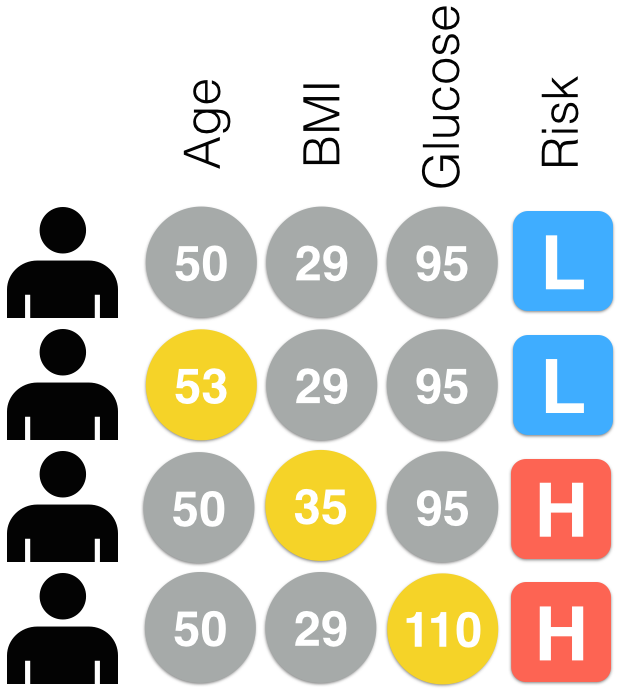
\includegraphics[width=0.3\linewidth]{prospector/local-inspection-explanation} % 0.3
\caption{
This illustration provides an explanation of how local inspection works.  On the top row are the patient's original feature values and the corresponding prediction.  On the bottom three rows, users changed certain values of the patient, highlighted in yellow, and such values impacted the prediction.
}
\label{figs:liexplain}
\end{figure}

Our second core contribution is leveraging our implementation of partial dependence to support the user task of local inspection.  Users can use \prospector to inspect specific data points of interest and see how the models predict how they behave.  In addition, if the users are curious about how a particular data point's risk might change if it had different values, a user can explore this as well.  The idea of localized inspection is illustrated in Figure~\ref{figs:liexplain} using our running example of Diabetes prediction.  At the top, the original patient's feature values are shown, along with the patient's original predicted low risk of having Diabetes. Suppose the analyst was curious to see how the patient's risk would change if his BMI was increased to 35.
Localized inspection allows users to interactively change this value, and see the corresponding prediction.
In order to streamline this kind of exploration we fully compute the
predicted risk for all values of BMI similar to partial dependence.
As seen in Figure~\ref{figs:liexplain} we do this for all features independently
yielding local partial dependence plots for each feature using a single input row.
% Using the idea of partial dependence on a single row of the input data set creates a localized partial dependence describing the axis aligned neighborhood of one point in the prediction function. This enables what-if scenarios by changing some values of the input row and seeing how the predicted outcome changes.

\begin{figure}
\centering
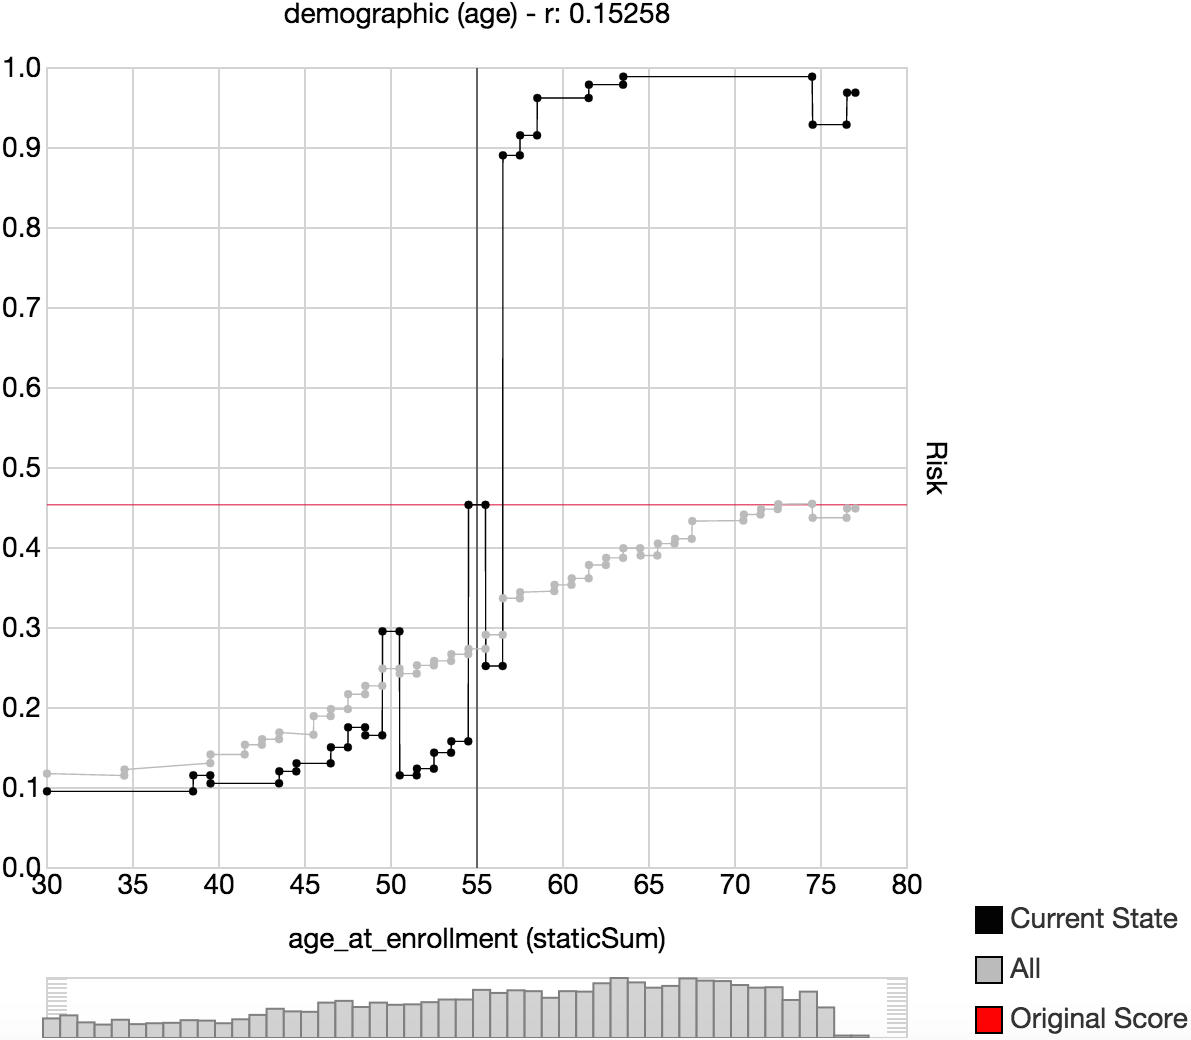
\includegraphics[width=0.8\linewidth]{prospector/compress_1} \\  \vspace*{0.2em} % 0.8 no vs
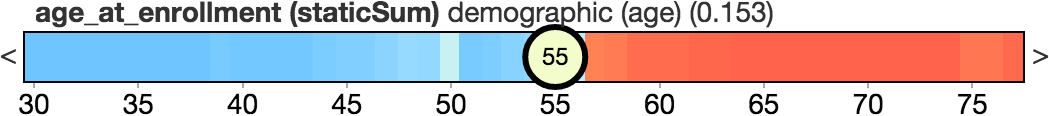
\includegraphics[width=0.9\linewidth]{prospector/compress_2} \\  \vspace*{0.5em} % 0.9 no vs
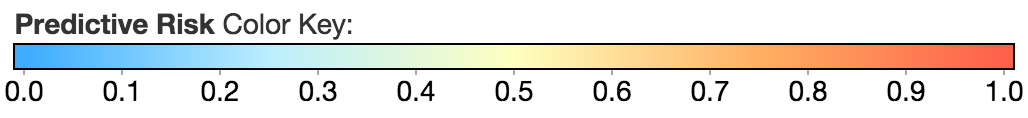
\includegraphics[width=0.7\linewidth]{prospector/color_scale} % 0.7
\caption[The same feature shown as line plot and partial dependence bar.]{
The same feature shown as line plot (top) and partial dependence bar (middle).
Color indicates the predicted risk for the outcome.
The color mapping is shown at the bottom.
}
\label{figs:compress}
\end{figure}

\subsubsection{Partial Dependence Bars}
In order to increase interactivity, encourage exploration, and display a larger number of features at once, we use a novel visual encoding, \emph{partial dependence bars}, a color bar representation of a partial dependence plot, shown in Figure~\ref{figs:compress}. The horizontal axis of a partial dependence bar represents the range of values of a feature, and the color at a given position represents the predicted risk for that value.  Color is mapped to a three-point color scale, where blue represents low risk, yellow represents medium risk, and red represents high risk.  As these bars are meant to aid local inspection, the current feature value of the datapoint being inspected is positioned along the horizontal axis and annotated as a circular label.  Users can drag this circular label left or right to inspect how changes in the feature value affect the predicted risk as well as the local partial dependence of other features.

\subsubsection{Local Feature Importance}
The fourth novel contribution of our research is a technique to simplify the
exploration of the predicted risk space by automatically finding features where a small change in value yields a significantly large change on the predicted risk.

While manipulating values of specific features allows users to test hypotheses on how features of interest may impact the prediction, if users wish to simply understand how to most impact the prediction, manipulating features one-by-one to test impact is an inefficient process.  Instead, \prospector can employ local feature importance, a novel technique that computes the impact of a given feature on the model according to the current values.  This localized feature importance comes in two different flavors: as a feature importance number and as actual suggestions for value changes.

A straight-forward way to define a localized importance of features is to look at the range of possible
predicted risks the feature can create starting from the given data point.
Formula (\ref{eq:importance}) computes the local importance $I$ of a given feature $f$ for the given feature
vector $p$. It sums up the entirety of changes in outcomes for all values $v$ for feature $f$.
The outcome changes are weighted by $\omega$ the likelihood of changing the value from $p_f$ to $v$.
$p^{\ast}$ is the modified feature vector where its value for $f$ is set to $v$ and $pred$ is the prediction function.

\begin{equation}
I_{f}(p) = \int_{-\infty}^{\infty}
\left[ pred(p^{\ast}) - pred(p) \right] \; \omega(v, \, p_f) \; dv
\label{eq:importance}
\end{equation}%
\[
\text{with}\; p^{\ast}_{f} = v \;\text{and}\; p^{\ast}_{g} = p_{g} \;\text{for}\; g \neq f
\]\[
\omega(v, \, p_f) = \frac{1}{\sigma_f \sqrt{2\pi}}
\exp \left( -\frac{(v - p_f)^2}{2\sigma_f^2} \right)
\]

In order for different features to be comparable, $\omega$ takes the distribution of values in the input data
into account. In features with a high spread, a larger change is more likely than in a feature with a narrow value range.
We model the likelihood of the change using a normal distribution with the reference value $p_f$ as mean and the
standard deviation $\sigma_f$ of the observed values of $f$ as standard deviation.
Ordering the features according to this local importance yields features that are likely to
decrease the predicted risk first, then features that have a low impact on the predicted risk,
and finally features that are likely to increase the predicted risk.

% \subsubsection{Local impact suggestions}
Instead of computing local feature importance for all possible changes, it is more
practically useful to compute the importance according to the most \emph{impactful} change for a feature.
An impactful change is the smallest change needed to have the largest change in the predicted outcome.
Note that this is different from the slope of the function since an impactful change
might be after a valley or ridge. Again, in order to have comparable
results, the distribution of values in the input data is taken into account.

\begin{equation}
\argmax_v \left[
s \; \left[ pred(p^{\ast}) - pred(p) \right] \; \omega(v, p_f)
\right]
\label{eq:impact}
\end{equation}

Formula (\ref{eq:impact}) finds the most impactful change of a feature.
$s$ is either $1$ or $-1$ depending on whether to search for the largest increase or decrease.
All other variables are the same as in Formula (\ref{eq:importance}).
The changes yielding the highest impact can be interpreted as suggestions for changing a data point.

\begin{figure}[t]
\centering
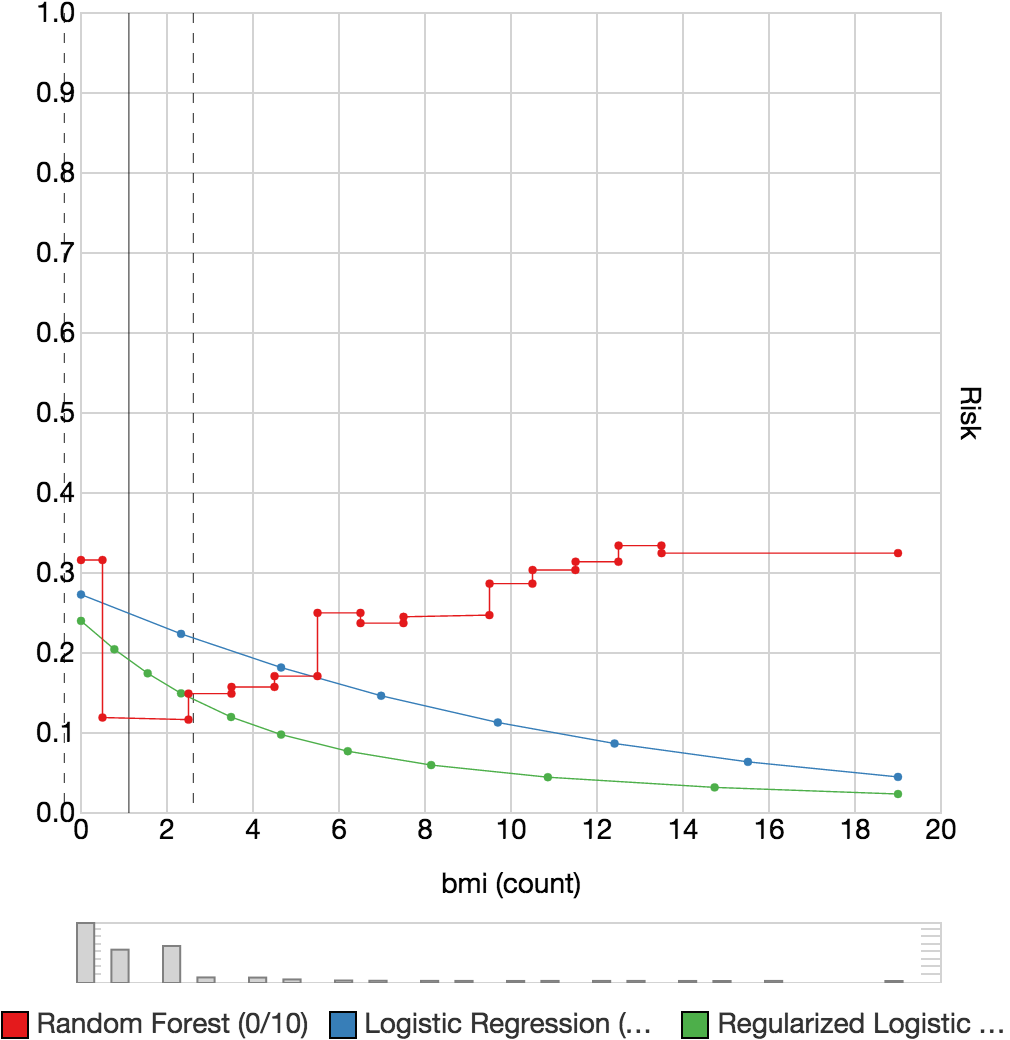
\includegraphics[width=0.7\linewidth]{prospector/cmp_bmi} % 0.8
\caption{
Comparison of three machine learning models on the number of measured BMI values.
The two regression models (logistic regression in blue and regularized logistic regression in green)
can express only a single slope (downwards or upwards) whereas the random forest in red can
model the strong decrease in predicted risk going from no BMI measures to one measure as well as
the later increase again if a patient has several BMI measures.
The random forest is more expressive, but the distribution of input values in the histogram below the plot hint the model might be overfitting as most of the observed values are 2 or less.
}
\label{figs:cmp_bmi}
\end{figure}
